\documentclass{ieeeaccess}
\usepackage{cite}
% Slightly tighter float-to-text separation (within IEEE norms) to satisfy
% the 12-page budget; content and float placement are unchanged.
\setlength{\textfloatsep}{13pt plus 2pt minus 4pt}
\setlength{\dbltextfloatsep}{13pt plus 2pt minus 4pt}
\usepackage{url}
% Allow URL line breaks at common URL separators to prevent overflow
\makeatletter
\g@addto@macro\UrlBreaks{\do\/\do\-\do\.\do\_\do\?\do\&\do\=\do\#\do\:}
\makeatother
\usepackage{amsmath,amssymb,amsfonts}
\usepackage{algorithmic}
\usepackage{graphicx}
\usepackage{textcomp}
\usepackage{booktabs}

% Relax float placement to keep figures near their citations
\renewcommand{\topfraction}{0.95}
\renewcommand{\bottomfraction}{0.8}
\renewcommand{\textfraction}{0.05}
\renewcommand{\floatpagefraction}{0.6}
\renewcommand{\dbltopfraction}{0.95}
\renewcommand{\dblfloatpagefraction}{0.6}

\def\BibTeX{{\rm B\kern-.05em{\sc i\kern-.025em b}\kern-.08em
T\kern-.1667em\lower.7ex\hbox{E}\kern-.125emX}}

% Override IEEE Access template placeholder for volume/year (class defaults: vol 11, 2023)
\def\thevol{00}
\def\theyear{2026}

\begin{document}
    \history{Date of publication xxxx 00, 0000, date of current version xxxx 00, 0000.}
    \doi{10.1109/ACCESS.XXXXXXXXX}

    \title{Posterior-Aware Online Matching of EV--Charger Pairs under Delayed Anonymous Telemetry}

    \author{\uppercase{Jiseok Yang}\authorrefmark{1},
        \uppercase{Daisuke Kodaira}\authorrefmark{2}, \IEEEmembership{Member, IEEE}}

    \address[1]{Degree Programs in Systems and Information Engineering, Graduate School of Science and Technology, University of Tsukuba, Tsukuba 305-8573, Japan}
    \address[2]{Institute of Systems and Information Engineering, University of Tsukuba, Tsukuba 305-8573, Japan}

    \tfootnote{This work was supported by the Human Security Collaboration (HSC) Projects, University of Tsukuba.}

    \markboth
    {Yang \headeretal: Posterior-Aware Online Matching of EV--Charger Pairs under Delayed Anonymous Telemetry}
    {Yang \headeretal: Posterior-Aware Online Matching of EV--Charger Pairs under Delayed Anonymous Telemetry}

    \corresp{Corresponding author: Daisuke Kodaira (e-mail: kodaira.daisuke.gf@u.tsukuba.ac.jp).}

                    \begin{abstract}
        The rapid adoption of electric vehicles is increasing the importance of smart charging and vehicle-to-grid operation, both of which require the charging backend to identify the vehicle connected to each charger. However, widely deployed International Electrotechnical Commission 61851-based alternating-current chargers do not provide vehicle identity through the charging interface, leaving EV--charger associations unavailable in multi-port charging environments. Prior experimental current-modulation studies infer these links by comparing charger-side current commands with vehicle-side current responses, but they assume a static batch setting with simultaneous sessions and complete current waveforms. Accordingly, this paper formulates the task as an online one-to-one matching problem under asymmetric observability. In this setting, EV sessions arrive and depart asynchronously, and EV-side telemetry is delayed, anonymous, coarsely sampled, and affected by sensing noise and packet loss. To address these challenges, we propose a two-stage Bayesian posterior matcher that integrates timing and current-response evidence through sequential posterior updates within each watermark decision. The method is evaluated in a 12-h event-driven online simulation with 50 charging ports and 500 EV sessions. Under identical decision timing in the evaluated simulation setting, the method achieves an average identification accuracy of 0.97, outperforming timing-based and waveform-based baselines. These simulation results show that the proposed method extends current-modulation-based EV--charger association recovery from static batch processing to online identification under asynchronous charging sessions and delayed anonymous telemetry.
    \end{abstract}

    \begin{keywords}
        Battery chargers, Bayes methods, Electric vehicles, Pattern matching, Telemetry, Vehicle-to-grid.
    \end{keywords}

    \titlepgskip=-15pt

    \maketitle

    \section{INTRODUCTION}

    The rapid growth of electric vehicle (EV) adoption worldwide~\cite{biea26} is making charging infrastructure an active interface between mobility demand and power-system operation rather than a passive energy-delivery layer.
    Smart charging and vehicle-to-grid (V2G) operation are expected to help manage this transition by shifting, limiting, or reversing charging power in response to grid conditions~\cite{b2,b3,b5}, but they require the charging backend to know which physical vehicle is connected to each active charger.

    Alternating-current (AC) chargers remain widely deployed due to lower hardware cost and simpler installation~\cite{b8}.
    Most operate under International Electrotechnical Commission (IEC) 61851-1, where the charger communicates only a maximum allowable current to the EV through the pulse-width-modulated control pilot, with no exchange of vehicle identity~\cite{biec,b6}.
    More advanced standards such as ISO~15118 can support vehicle identification and plug-and-charge~\cite{b7}, but their deployment will not immediately cover the large installed base of legacy AC chargers and EVs.
    This communication constraint creates a pair-level missing-link problem at multi-port charging sites: the backend knows which Electric Vehicle Supply Equipment (EVSE) slots are active and which command-current profiles are being issued to them, but it cannot directly determine which physical EV occupies each slot, undermining per-vehicle billing, V2G dispatch addressing, and verification of vehicle-side telemetry against charger-side records.

    To recover this missing link without adding new communication hardware, Baba and Imanaka~\cite{b13} introduced Modulated Charging Current Technology (MCCT), which modulates the charger-side allowable current and infers the EV--charger association by comparing the charger-side reference with the EV-side current response.
    Nomura~\textit{et al.}~\cite{b14} extended MCCT to static multi-pair matching on a Wallbox Pulsar Plus AC charger and a Tesla Model~3 RWD Standard Range Plus setup.
    Their data-driven current-generation model was built from console command values, charger-cloud current measurements, and EV-cloud current measurements, and it included sampling intervals, command-to-measurement delays, and a charger--EV current-shape offset.
    Using correlation--Euclidean and correlation--dynamic-time-warping (DTW) cost matrices solved by the Hungarian method~\cite{b15}, they reported pairing accuracy above 99\% for 300 simultaneous pairs at a 30\,s EV sampling interval.

    This prior evaluation provides the measurement-based foundation for the present work, but its identification setting remains static: all EV--charger pairs are assumed to start simultaneously, the relevant waveforms are available when the cost matrix is constructed, and the assignment is solved as a one-shot batch problem.
    In actual cloud-connected operation, EV sessions arrive and depart asynchronously, and EV-side observations become available only as delayed, anonymous, and imperfect telemetry.
    The problem therefore shifts from static waveform assignment over completed traces to online identification from maturing evidence.

    This paper extends prior measurement-based MCCT modeling from static batch assignment to online pair identification under asynchronous sessions and delayed anonymous EV-side telemetry.
    It formulates the task as a sequential online one-to-one matching problem under asymmetric observability and proposes a two-stage Bayesian posterior matcher (hereafter the Posterior matcher) that combines timing and waveform evidence through a two-stage posterior update before watermark-based finalization, where the \emph{watermark}, an event-time data-maturity rule~\cite{b26}, declares when delayed telemetry is complete enough to decide.
    The contribution is not Bayesian updating alone; it is an online MCCT formulation under two-plane asymmetric observability, combined with a sequential posterior decision rule that carries belief across update stages and is evaluated at a shared watermark.

    The main contributions of this paper are as follows:
    \begin{enumerate}
        \item We formulate MCCT-based EV--charger identification as an online one-to-one matching problem under delayed anonymous telemetry.
        \item We extend a measurement-based Wallbox--Tesla current-generation model to an event-driven online runtime.
        \item We propose and evaluate a two-stage Bayesian posterior matcher that achieves 0.97 identification accuracy in a representative 500-session scenario and improves over timing-only and waveform-based baselines.
    \end{enumerate}

    The remainder of this paper is organized as follows.
    Section~II reviews related work on EV identification, online assignment, online evidence integration, and delayed telemetry.
    Section~III formalizes the system model and online one-to-one decision problem.
    Section~IV presents the shared runtime and the four compared matchers.
    Section~V describes the simulation environment and ingestion model.
    Section~VI reports the comparative evaluation, sensitivity sweeps, and ablation results.
    Section~VII concludes the paper.

    \begin{figure*}[!t]
        \centerline{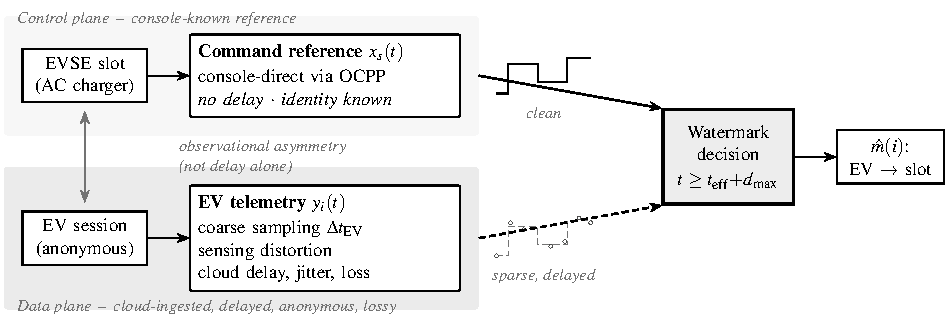
\includegraphics[width=\textwidth]{figure1_two_plane_observability.pdf}}
        \caption{Two-plane observability in the proposed EV--charger matching problem. The control plane (EVSE-side MCCT reference $x_s(t)$) is read directly from the OCPP console without uplink delay, whereas the data plane (EV-side telemetry $y_i(t)$) reaches the backend after sensing distortion, cloud-ingestion delay, jitter, and loss. This observational asymmetry, not delay alone, is the defining feature of the problem and necessitates the online matching formulation developed in this paper. Finalization fires at $t \geq t_{\text{eff}} + d_{\max}$, the effective session end plus the watermark delay bound (Section~III-B); {\unboldmath$\Delta t_{\text{EV}}$} is the EV sampling period.}
        \label{fig01}
    \end{figure*}
    \section{RELATED WORK}

    Smart charging and V2G operation require the charging backend to associate each connected EV with its EVSE slot~\cite{b2,b3,b5}.
    Prior work related to this requirement falls into three groups: EV identification from charging behavior, matching and assignment within EV charging systems, and online evidence integration under delayed telemetry.
    However, these studies do not directly resolve the present setting, where the EV--EVSE association must be recovered online from delayed, anonymous, and imperfect EV-side telemetry on legacy IEC~61851 AC infrastructure.

    \subsection{EV Identification From Charging Behavior}
    Non-intrusive load monitoring~\cite{bhart} established that an electrical load carries identifying information.
    EV charging in particular produces repeatable and discriminative patterns at the distribution-feeder level~\cite{b9} and at the session-data level, supporting brand-and-model classification~\cite{b10}, per-vehicle fingerprinting~\cite{b11}, and session-duration-class classification~\cite{b12}.
    Recent work pushes this further toward earlier and finer-grained EV-instance recognition from early-charging voltage patterns~\cite{bmarchiori25}.
    Adjacent results extract related vehicle-state information from charging signals, including AC reference-power tracking~\cite{bferretti24} and state-of-charge estimation~\cite{b20,b21}.
    These studies confirm that charging signals carry vehicle-level information, but they answer \emph{what kind of vehicle} or \emph{which previously enrolled vehicle} is being charged.
    They do not answer the operational pair question of \emph{which of several concurrently active EVs is on which EVSE slot} from delayed, anonymous cloud telemetry alone.

    \subsection{Matching and Assignment in EV Charging Systems}
    EV-charging-specific matching has been studied for several operational questions, including stable matching for subscription-based service models~\cite{bkhanda} and capacity-aware top trading cycles for post-choice reassignment in shared cyber-physical charging environments~\cite{breactttc}.
    These works presume declared user preferences, known vehicle identities, and timely coordination channels, and frame the operational question as how to \emph{allocate} or \emph{reassign} EVs across stations.
    The present setting is not an allocation problem in that sense: the EV is already physically connected, and the task is to \emph{recover} the missing physical-to-logical pair link from anonymous, delayed, waveform-only evidence.

    \subsection{Sequential Association and Delayed Telemetry}
    The methodological tools for committing one-to-one decisions under partial and uncertain evidence are well established.
    Online bipartite matching~\cite{b17,b18}, with recent extensions for decision deferral under delayed information~\cite{bemek16}, supplies the formal assignment basis.
    Recursive Bayesian filtering~\cite{b19,bsarkka} motivates the posterior-updating mechanism used in this work, applied here to anonymous, asymmetric, delay-bounded EV-current telemetry rather than to spatially resolved, time-synchronous measurements.

    A parallel telemetry-side literature characterizes the delay envelope within which an online matcher must decide.
    The Open Charge Point Protocol (OCPP)~\cite{b22}, the underlying WebSocket~\cite{b23} over Transmission Control Protocol (TCP)~\cite{b24} transport, and broadband-latency baselines~\cite{b25} motivate bounded low-second-scale ingestion assumptions.
    Formal watermark semantics from event-time stream processing~\cite{b26} then supply the rule by which delayed evidence is judged mature enough for irrevocable finalization.
    This strand quantifies delay, jitter, and maturity in isolation, but does not address how to integrate the resulting delayed evidence into a strict one-to-one EV--EVSE assignment.

    Taken together, the three strands offer vehicle-level information, an assignment basis, and a method for online integration of uncertain evidence, but none combines them for pair-level EV--EVSE identification in the present setting.
    The present work addresses this gap by integrating timing and waveform evidence through a staged posterior decision rule inside a shared event-driven runtime and finalizing under a data-maturity rule.

    \section{SYSTEM MODEL AND PROBLEM FORMULATION}

    Building on the measurement-based current-generation model used in prior MCCT work~\cite{b14}, this section defines the additional online decision layer required when EV-side observations are not available as a complete batch but arrive through delayed anonymous telemetry.
    The runtime layer introduced here is shared by all matchers compared in Section~IV and underlies the experimental envelope defined in Section~V.

    \subsection{Operational Objective and Two-Plane Observability}
    Let $i \in E$ denote an EV session and $s \in S$ denote an EVSE slot, where $E$ and $S$ are the session and slot sets.
    The operational objective is to emit an online finalized mapping $\hat{m}(i) \in S$ that matches the true EVSE slot of session $i$, with one-to-one consistency enforced among simultaneously finalized matches.
    Each EVSE slot is physically exclusive: at any time $t$, slot $s$ hosts at most one session, so for any two sessions $i \neq j$ admitted to the same slot ($m(i) = m(j) = s$, where $m$ denotes the true admission mapping) the active intervals $[t_{\text{arr},i}, t_{\text{end},i}]$ (from arrival $t_{\text{arr},i}$ to session end $t_{\text{end},i}$) are disjoint.
    An arriving EV is admitted to a slot that is free at $t_{\text{arr},i}$; admission scheduling is therefore not a degree of freedom of the matcher.

    The system model contains two observation planes (Fig.~\ref{fig01}) that explicitly separate the EVSE-side reference (control plane, console-direct) from the EV-side telemetry (data plane, cloud-ingested).
    This separation is conceptually consistent with the information-and-communication-technology (ICT)--energy-equipment decomposition reference model of Imanaka~\textit{et al.}~\cite{bimanaka23} and with the broader edge-cloud architectural perspective of Satyanarayanan~\cite{bsatya}.
    The control plane provides the console-known EVSE reference stream $x_s(t)$ for each slot $s$.
    The reference is generated from the MCCT command pattern through the data-driven model in Section~V-A.
    The charger is remotely commanded via OCPP, and the charger-cloud log is directly accessible at the control console~\cite{b14}.
    This stream is therefore treated as known without uplink delay.
    The data plane provides an anonymous EV observation stream $y_i(t)$ for each EV session $i$.
    The stream is observed only after asynchronous ingestion with the impairments described in Section~V-A.
    The two-plane asymmetry---not delay alone---is the defining feature of this problem.

    \subsection{Window--Watermark Online Decisioning}
    The MCCT observation window has duration
    \begin{equation}\label{eq:e1}
        W = \tau \cdot N_{\text{steps}},
    \end{equation}
    where $\tau = 60$\,s and $N_{\text{steps}} = 6$, yielding $W = 360$\,s.
    This window length follows the MCCT observation convention of prior work~\cite{b13},~\cite{b14}, keeping the matching task directly comparable.
    The nominal decision-window end is $t_{\text{win},i} = t_{\text{arr},i} + W$.
    The runtime does not, however, finalize exactly at $t_{\text{win},i}$ because EV-side telemetry may still be in transit.
    Instead, it waits until a watermark condition is satisfied: in event-time stream processing, a watermark marks the time by which all records with earlier event times are assumed to have arrived~\cite{b26}; here it bounds when the delayed EV-side prefix of session $i$ is complete enough for an irrevocable pairing decision.
    Let $d_{\max}$ denote the watermark delay bound.
    The watermark-ready time is
    \begin{equation}\label{eq:e2}
        t_{\text{wm},i} = t_{\text{eff},i} + d_{\max},
    \end{equation}
    where the effective end time is defined as
    \begin{equation}\label{eq:e3}
        t_{\text{eff},i} = \min\!\left(t_{\text{arr},i} + W,\; t_{\text{end},i}\right),
    \end{equation}
    where $t_{\text{end},i}$ is the end timestamp reported by the anonymous EV-side stream itself (which carries a session identifier and boundaries but no EVSE-slot label), not a charger-side ground-truth endpoint. The $\min$ clamp advances the watermark to the actual end when a session closes before the nominal window, preventing the watermark from overshooting into a future that will never be observed.
    An EV session is mature when $t \geq t_{\text{wm},i}$, which bounds waiting: deciding too early yields a too-short EV prefix, waiting too long degrades online usefulness.

    \subsection{Candidate Gating, Assignment, and Finalization Semantics}
    The candidate slot set for EV session $i$ is restricted to slots active near the effective end.
    Let $\Delta$ denote the candidate time margin.
    Then
    \begin{equation}\label{eq:e4}
        C_i = \{ s \in S \mid s \text{ active within } [t_{\text{eff},i} - \Delta, \; \min(t_{\text{eff},i} + \Delta,\; t_{\text{wm},i})] \}.
    \end{equation}
    Candidate gating reduces computational burden and narrows matching to operationally plausible slots; the upper bound is clamped at the watermark-ready time $t_{\text{wm},i}$ so that gating never uses slot activity observed after the decision, preserving online causality.
    If $C_i$ is empty, the runtime falls back to the full EVSE-slot set $S$ and records the fallback invocation (which remains zero in the base-load regime).
    When several mature EV sessions are processed together, the runtime constructs a cost matrix $\mathbf{C} = [c_{i,s}]$ (distinct from the candidate set $C_i$) and solves
    \begin{equation}\label{eq:e5}
        \min_\pi \sum_i c_{i,\pi(i)} \quad \text{s.t.} \quad \pi(i) \in C_i,\; \pi(i) \neq \pi(j)\;\text{for}\;i \neq j.
    \end{equation}
    The compared algorithms differ in how $c_{i,s}$ is computed, and the finalized mapping emitted by the runtime satisfies $\hat{m}(i) = \pi(i)$.
    An EV session is \textit{admitted} if it can be scheduled onto an available EVSE slot, and \textit{blocked} if no capacity is available.
    A session is \textit{finalized} when the runtime emits an EV--charger match.
    Finalization occurs through ordinary watermark-based maturity or, in rare cases, through fallback logic.
    The watermark maturity rule, candidate gating in Eq.~\eqref{eq:e4}, and per-batch one-to-one finalization are shared by all four matchers studied in Section~IV.
    Matcher-specific extensions are limited to the Posterior matcher, which builds a per-session posterior through two update stages before assignment costs are computed.

    \subsection{Evaluation Metrics}
    Three primary metrics are reported: overall identification accuracy $\tfrac{N_{\text{correct}}}{N_{\text{admitted}}}$, requested-session accuracy $\tfrac{N_{\text{correct}}}{N_{\text{requested}}}$, and 90th-percentile decision latency $\text{Quantile}_{0.9}(\{t_{\text{final},i} - t_{\text{arr},i}\})$, where $N_{\text{requested}}$ counts all arriving sessions (admitted plus blocked) and $t_{\text{final},i}$ is the finalization time; the first two coincide at low load and diverge only under saturation, where requested-session accuracy becomes the operationally meaningful measure, and candidate-set composition (average count, ground-truth retention, fallback invocations) is recorded as auxiliary diagnostic.

    \begin{figure*}[!t]
        \centerline{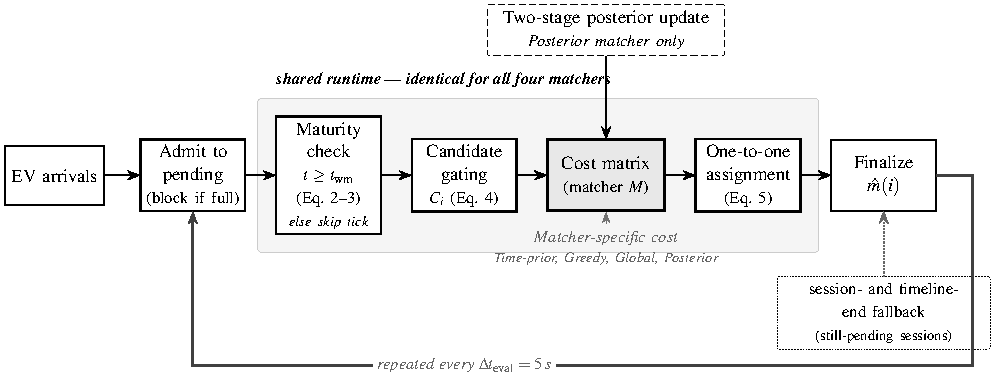
\includegraphics[width=\textwidth]{figure2_event_driven_runtime.pdf}}
        \caption{Shared event-driven runtime used by all compared matchers. The entire loop---arrivals, maturity, candidate gating, cost-matrix construction, assignment, and finalization---re-runs at every evaluation tick ({\unboldmath$\Delta t_{\mathrm{eval}} = 5$\,s}). All four matchers use identical watermark maturity, candidate gating, batch construction, and per-batch one-to-one finalization timing; they differ only in cost-matrix construction. The Posterior matcher additionally applies a two-stage posterior update before constructing the cost matrix.}
        \label{fig02}
    \end{figure*}

    \section{PROPOSED AND BASELINE MATCHERS}

    This section presents the four matchers compared in this study, all of which operate inside the shared event-driven runtime introduced in Section~III.

    \subsection{Event-Driven Runtime}
    The runtime is explicitly event-driven with evaluation interval $\Delta t_{\text{eval}} = 5$\,s.
    At each evaluation tick the runtime updates the pending session set, checks maturity via $t_{\text{wm}} = t_{\text{eff}} + d_{\max}$ with $t_{\text{eff}}$ clamped per Eq.~\eqref{eq:e3}, constructs candidate slot sets via Eq.~\eqref{eq:e4} with margin $\Delta$, evaluates pairwise compatibility on the watermark-visible prefix, builds a cost matrix over the matured batch, and solves one-to-one assignment.
    Two fallback paths are supported: session-end (a session ends before watermark readiness) and timeline-end (pending sessions at scenario termination). In the main base-load regime the fallback ratio remains zero.
    Fig.~\ref{fig02} shows this shared loop; its shared band marks the components common to all four matchers---watermark maturity, candidate gating, batch construction, and the assignment solver---isolating the cost-matrix block as the only divergence point among Time-prior, Greedy, Global, and Posterior.
    With maturity, gating, and timing held identical, the accuracy differences reported in Section~VI are attributable to cost construction and belief-update differences.

    \subsection{Baseline and Proposed Matchers}
    Four methods share watermark maturity, candidate gating, and per-batch decision timing.
    The Time-prior, Greedy, and Global matchers are single-shot decisions that differ only in cost-matrix construction.
    The Posterior matcher additionally uses a two-stage posterior update before the shared assignment step (TABLE~\ref{table2}).
    Within the present runtime, the posterior-carry-over-removed ablation in Section~VI-C reduces the proposed matcher to a single-step Bayesian scorer without sequential state, isolating the contribution of sequential posterior integration relative to a memoryless Bayesian update.

    \begin{table}[htbp]
        \caption{Matcher design summary. Only the Posterior matcher uses an explicit two-stage posterior update, separating it structurally from the single-shot baselines.}
        \label{table2}
        \centering
        \setlength{\tabcolsep}{3pt}
        \scriptsize
        \begin{tabular}{@{}l p{2.1cm} p{1.5cm} p{1.3cm}@{}}
            \toprule
            \textbf{Matcher} & \textbf{Primary evidence} & \textbf{Assignment} & \textbf{Posterior update} \\
            \midrule
            Time-prior & Timing only & Hungarian & None \\
            Greedy & DTW + step-sig. & Greedy 1:1 & None \\
            Global & Correlation + DTW & Hungarian & None \\
            Posterior & Bayesian posterior & Hungarian & Two-stage \\
            \bottomrule
        \end{tabular}
    \end{table}

    \textbf{Time-prior baseline.}
    The time-prior baseline is a timing-only reference that ignores waveform shape entirely; compatibility is the temporal-proximity cost
    \begin{equation}\label{eq:a0}
        c^{(A0)}_{i,s} = D_{\text{end}}(t_{\text{eff},i}, s) + 0.10\,D_{\text{start}}(t_{\text{start\_est},i}, s),
    \end{equation}
    where $D_{\text{end}}$ is the minimum distance from $t_{\text{eff},i}$ to any slot-$s$ active boundary and $D_{\text{start}}$ is the minimum distance from the EV start-estimate to any slot-$s$ active start, after which Hungarian assignment is applied.
    It is a quantitative anchor rather than a competitive method; its gap to the other three matchers isolates the value of waveform evidence.

    \textbf{Greedy waveform matcher.}
    The greedy waveform matcher evaluates a pairwise cost from the EV prefix and the EVSE-slot prefix:
    \begin{equation}\label{eq:e6}
        c^{(A1)}_{i,s} = \lambda_{\text{dtw}}\,d^{\text{dtw}}_{i,s} + \lambda_{\text{step}}\,d^{\text{step}}_{i,s} + \lambda_{\text{mean}}\,d^{\text{mean}}_{i,s},
    \end{equation}
    where $d^{\text{dtw}}$ is a band-constrained DTW discrepancy~\cite{b16} computed on z-normalized prefixes and divided by the prefix length, $d^{\text{mean}}$ is the mean-gap term, and $d^{\text{step}}$ is the step-signature discrepancy computed on per-step medians as
    \begin{equation}\label{eq:e7}
        d^{\text{step}}_{i,s} = \text{mean}|e_{\text{sig}} - s_{\text{sig}}|,
    \end{equation}
    in which $e_{\text{sig}}$ and $s_{\text{sig}}$ are step medians (in amperes) over each $\tau$-second sub-window, so $d^{\text{step}}$ is in amperes and penalizes local mismatch on the same temporal grid as the MCCT step pattern.
    The default constants are $\lambda_{\text{dtw}} = 1.0$, $\lambda_{\text{step}} = 0.40$, $\lambda_{\text{mean}} = 0.0$; calibration on the calibration slice (Section~V-C) showed $d^{\text{mean}}$ to be subsumed by the DTW term at this sampling rate, so the Greedy matcher effectively operates on DTW plus the step-signature cost.
    Candidate pairs are sorted by cost and selected greedily under one-to-one uniqueness constraints, providing a lightweight waveform baseline.

    \textbf{Global waveform assignment.}
    The global waveform assignment computes a combined waveform score from normalized correlation $\rho^{\text{norm}}$ and normalized DTW $\delta^{\text{norm}}$:
    \begin{equation}\label{eq:e8}
        \text{eval}_{i,s} = \rho^{\text{norm}}_{i,s} \cdot \delta^{\text{norm}}_{i,s},
    \end{equation}
    \begin{equation}\label{eq:e9}
        c^{(A2)}_{i,s} = 1 - \text{eval}_{i,s}.
    \end{equation}
    Correlation is mapped from $[-1, 1]$ to $[0, 1]$ via
    \begin{equation}\label{eq:rhonorm}
        \rho^{\text{norm}} = \frac{\rho + 1}{2}.
    \end{equation}
    The DTW distance is first normalized by the alignment-path length to remove sequence-length bias.
    It is then min--max scaled across the finite candidate pairs of the matured batch (when all values coincide, $\delta^{\text{norm}} = 1$ for every pair), giving the normalized similarity
    \begin{equation}\label{eq:deltanorm}
        \delta^{\text{norm}} = 1 - \text{MinMax}(\text{DTW}_{\text{path}}).
    \end{equation}
    The resulting dense cost matrix is passed to Hungarian assignment~\cite{b15}.

    \textbf{Two-stage posterior matcher.}
    The two-stage posterior matcher is a runtime-integrated Bayesian matcher designed for anonymous, delayed EV telemetry under global one-to-one constraints.
    At each watermark decision for a mature batch, it performs two posterior-update stages over each candidate set.
    Following recursive Bayesian filtering~\cite{b19},~\cite{bsarkka}, update stage $k$ combines a timing prior $P_t(s|i)$, a current-based likelihood $P_c(s|i)$, and the previous within-decision posterior $P_{k-1}(s|i)$ through
    \begin{equation}\label{eq:e10}
        P_k(s|i) \propto P_{k-1}(s|i)^{\gamma_{\text{prev}}} \cdot P_t(s|i)^{\gamma_t} \cdot P_c(s|i),
    \end{equation}
    where $\gamma_{\text{prev}}$ and $\gamma_t$ weight the within-decision carry-over belief relative to the current stage's waveform evidence.
    The current-based likelihood is a scale-normalized softmax over the candidate set,
    \begin{equation}\label{eq:pc}
        P_c(s|i) = \frac{\exp\!\big(-\beta_{\text{curr}}\,\frac{c_{i,s}-c_i^{\min}}{\sigma_i}\big)}{\sum_{s'\in C_i}\exp\!\big(-\beta_{\text{curr}}\,\frac{c_{i,s'}-c_i^{\min}}{\sigma_i}\big)},
    \end{equation}
    where $c_{i,s}$ is the refined DTW and step-signature waveform cost (cf.\ Eq.~\eqref{eq:e6}--\eqref{eq:e7}) on the watermark-visible prefix, $c_i^{\min}=\min_{s\in C_i}c_{i,s}$, and $\sigma_i$ is the median absolute deviation of $\{c_{i,s}\}_{s\in C_i}$ (if it falls below $10^{-6}$, the standard deviation is used instead, then the value range, then unity); the two update stages evaluate $c_{i,s}$ on the first $60\%$ and on the full matured prefix, respectively (TABLE~\ref{table:hyper}).
    The time prior $P_t(s|i)$ is the temporal-overlap weight between the candidate slot's active interval and the EV-side window $[t_{\text{arr},i}, t_{\text{eff},i}]$: writing $\Delta\tau_{i,s}$ for the boundary distance and $q^{75}_i$ for the $75$th percentile of $\{\Delta\tau_{i,s}\}_{s\in C_i}$ (floored at 1\,s), the shaped prior is
    \begin{equation}\label{eq:shaped}
        P_t^{\text{shaped}}(s|i)\propto\exp\!\left(-\alpha_{\text{time}}\,\frac{\Delta\tau_{i,s}}{q^{75}_i}\right),
    \end{equation}
    blended with a uniform prior over $C_i$ as
    \begin{equation}\label{eq:ptblend}
        P_t = \eta_{\text{mix}}\,P_t^{\text{shaped}} + (1-\eta_{\text{mix}})\,P_t^{\text{uniform}},
    \end{equation}
    to prevent early posterior collapse on sparse evidence.
    At the first update stage ($k = 1$), the carry-over factor in Eq.~\eqref{eq:e10} is initialized as a uniform prior over $C_i$.
    Eq.~\eqref{eq:e10} is renormalized over $s \in C_i$ after every update.
    The $\alpha$, $\beta$, $\gamma$, and $\lambda$ hyperparameter family is listed in TABLE~\ref{table:hyper} together with the calibration basis.
    The implementation refines the posterior in two weighted stages per watermark decision, with stage-wise parameter values tabulated in TABLE~\ref{table:hyper}.
    Assignment costs blend the posterior log-cost with the last stage's current-likelihood log-cost,
    \begin{equation}\label{eq:e11}
        c^{(A3)}_{i,s} = (1 - \lambda_{\text{blend}})\,(-\log P_k(s|i)) + \lambda_{\text{blend}}\,(-\log P_c^{\text{last}}(s|i)),
    \end{equation}
    with $\lambda_{\text{blend}} = 0.15$ (TABLE~\ref{table:hyper}); $P_k$ is renormalized over $s \in C_i$ after each update.
    The Posterior matcher is the only method that constructs assignment costs from an explicit posterior state.

    \begin{table}[htbp]
    \caption{Hyperparameter values and calibration basis. All values are fixed on the calibration slice and frozen before any evaluation run.}
    \label{table:hyper}
    \centering
    \scriptsize
    \setlength{\tabcolsep}{3pt}
    \begin{tabular}{@{}l l p{4.2cm}@{}}
        \toprule
        \textbf{Symbol} & \textbf{Value} & \textbf{Calibration basis} \\
        \midrule
        $\lambda_{\text{dtw}}$ & $1.0$ & Unit-normalized weight on the DTW term \\
        $\lambda_{\text{step}}$ & $0.40$ & Selected on the calibration slice (Section~V-C) \\
        $\lambda_{\text{mean}}$ & $0.0$ & Mean-gap subsumed by DTW at this sampling rate \\
        $\gamma_{\text{prev}}$ & $0.60$ & Within-decision carry-over exponent (both stages) \\
        $\gamma_t^{(1)}$, $\gamma_t^{(2)}$ & $1.00$ and $0.20$ & Time-prior exponent at Stage~1 and Stage~2 \\
        $\alpha_{\text{time}}$ & $1.0$ & Timing-prior decay rate \\
        $\eta_{\text{mix}}$ & $0.35$ & Weight on shaped time-prior in $\eta_{\text{mix}}\,\text{shaped}+(1{-}\eta_{\text{mix}})\,\text{uniform}$ \\
        $\beta_{\text{curr}}$ & $1.0$ & Unit scale on current-based likelihood \\
        $\lambda_{\text{blend}}$ & $0.15$ & Small blend weight in $c^{(A3)}$ (Eq.~\eqref{eq:e11}); kept low so the posterior term dominates the blended cost \\
        \bottomrule
    \end{tabular}
    \end{table}

    \subsection{Hyperparameter Selection}
    The $\alpha$, $\beta$, $\gamma$, and $\lambda$ weights are fixed on a small held-out calibration slice and frozen before any evaluation run.
    The explicit calibration-versus-evaluation partition is given in Section~V-C, so the reported ranking is independent of the tuning signal.
    Numerical values of all hyperparameters are listed in TABLE~\ref{table:hyper} together with the calibration basis for each value.

    \section{EXPERIMENTAL SETUP}

    \subsection{Simulator and Signal Model}

    The simulation environment rests on three layers with decreasing empirical grounding: a measurement-based current-generation model that produces the charger-side and EVSE-side currents (Layer~1), an event-driven session-level runtime that schedules asynchronous EV arrivals and departures (Layer~2), and a cloud-ingestion model that determines how EV-side observations reach the backend (Layer~3).
    We do not replace the prior measurement-based current-generation model; rather, we embed it into an event-driven online runtime and add a cloud-ingestion layer that models delayed anonymous telemetry.
    Although the present study is simulation-based, its signal foundation is measurement-derived: Layer~1 reuses the data-driven current-generation model that Nomura~\textit{et al.}~\cite{b14} fitted to real Wallbox Pulsar Plus and Tesla Model~3 current measurements, so the simulated waveforms retain measured response features from that Wallbox--Tesla equipment pair rather than idealized step shapes.

    \textbf{Layer~1: Measurement-based current-generation model.}
    The charger-side command sequence follows a fixed six-step MCCT-style structure with $\tau = 60$\,s (yielding an observation window of $W = 360$\,s), and the EVSE-side reference is generated through the data-driven response model of Nomura~\textit{et al.}~\cite{b14}, fitted from EV and EVSE current measurements collected on a Wallbox Pulsar Plus AC charger and a Tesla Model~3 RWD Standard Range Plus under the original Baba--Imanaka equipment setup~\cite{b13}; as reported by Nomura~\textit{et al.}~\cite{b14}, these measurements were obtained from the YourStand AC charging-service deployment.
    The model captures three behaviors---delayed change onset, target-current offset, and asymmetric ramp---broadly consistent with real-world AC-charging current behavior reported in independent measurement-based studies~\cite{bferretti24}, and already incorporates measurement timing and current-shape offset effects observed in the Wallbox--Tesla setup.
    The command-to-current response lag used for waveform generation is modeled as 15\,s for the first nonzero charging step and 5\,s for subsequent setpoint changes.
    The 15\,s value is treated as a waveform-generation assumption informed by the EV charging full-activation-time (FAT) ranges reported by Imanaka and Baba~\cite{bimanaka25}.
    These values do not represent backend telemetry-arrival delay, which is modeled separately in the cloud-ingestion layer.
    The remaining fitted parameters are
    \begin{equation}\label{eq:e14}
        I_{\text{offset}} = 0.0221\,u + 0.2831,
    \end{equation}
    \begin{equation}\label{eq:e15}
        \Delta I_{\text{rise}} = 0.0327\,\Delta u + 0.3787,
    \end{equation}
    where $u$ is the commanded current setpoint (A), $\Delta u$ is the setpoint change between consecutive steps (A), $I_{\text{offset}}$ is the steady-state command-to-current offset (A), and $\Delta I_{\text{rise}}$ is the current rise rate (A/s).
    For falling transitions, the current decreases at a maximum rate of 4\,A per second, and the resulting EVSE current is rounded to 0.1\,A; this prevents the matching problem from being defined over an unrealistically ideal waveform.
    The EVSE reference sample interval is five seconds.

    \textbf{Layer~2: Online event-driven session model.}
    The online contribution of this study begins at the runtime layer: sessions are no longer assumed to be simultaneous or complete at the time of matching.
    The simulator configures a single site with fifty EVSE slots (charging ports) and a twelve-hour scenario horizon; the fifty-slot capacity provides a multi-port site setting for evaluating online matching under moderate candidate ambiguity, and together with sessions of ten to sixty minutes it keeps the evaluated EV-session count (up to 500 sessions) below saturation in the present envelope.
    Arrival times are sampled independently and uniformly over the first eleven hours of the horizon and then sorted. Session durations are sampled uniformly from ten to sixty minutes, inclusive. Each arriving session is admitted to a slot chosen uniformly at random among the slots free at its arrival time, using the seeded scenario random-number generator, under the slot-exclusivity constraint of Section~III-A; if no slot is free, the session is blocked.
    Each six-step command pattern starts at $0$\,A and is followed by five distinct setpoints drawn from $\{6,\dots,30\}$\,A, with a pairwise setpoint gap $\geq 4$\,A and a consecutive-step gap $\geq 8$\,A. The fifty per-slot patterns are selected from a seeded $3{,}000$-pattern pool by a farthest-point (maximin) procedure with a minimum pairwise $\ell_1$ setpoint distance $\geq 40$\,A. The reported accuracy is therefore conditional on this deliberately separated command codebook rather than on randomly sampled patterns.
    Within the present envelope (at most 500 sessions) the global capacity is never reached, so overall and requested-session accuracy coincide throughout the reported results; both are nonetheless retained because they diverge under saturation (future work).

    \textbf{Layer~3: Cloud-ingestion and telemetry imperfection.}
    The EV-side signal is formed by applying sensing distortion to the EVSE-side current: each sample is subject to additional sensing delay (max 20\,s) and start-estimate jitter (20\,s), and carries multiplicative gain variation (std~0.03), additive bias (std~0.35\,A), and additive noise (std~0.20\,A).
    Cloud-ingestion delay and packet loss follow an evidence-informed baseline: mean ingestion delay 2.0\,s, delay jitter (std) 1.0\,s, and packet-loss probability 0.005. These three values are engineering assumptions that fix a low-second-scale ingestion envelope, not field measurements of a specific EV-cloud service. The cited transport and broadband references~\cite{b23},~\cite{b24},~\cite{b25} motivate only the order of magnitude; because network round-trip is sub-second, the 2.0\,s mean represents application-level ingestion rather than transport delay. The 10.0\,s ingestion-delay cap follows the commercial OCPP MessageTimeout default~\cite{bzaptec},~\cite{b22} and is distinct from the decision-side watermark bound $d_{\max}$ of Eq.~\eqref{eq:e2}.
    The EVSE-side stream is not subjected to the same delay or loss model, since the control console is assumed to know the EVSE-side reference directly; this asymmetry is part of the problem definition.
    Four distinct delay quantities appear in the model and should not be conflated: the command-to-current response lag of the waveform-generation model (15\,s and 5\,s, Layer~1); the EV-side sensing and start-estimate delay (Layer~3 sensing distortion); the network cloud-ingestion delay (mean 2\,s, practical max 10\,s; TABLE~\ref{table3}); and the watermark bound $d_{\max}$ that governs when accumulated evidence is judged mature for finalization (Eq.~\eqref{eq:e2}). Only the watermark bound is a decision-side parameter; the other three delays describe how the EV-side evidence is generated and transported.
    The numerical results in Section~VI should be read as statements about this evaluation envelope and the ranking among the four matchers, not as absolute field predictions.

    \begin{table}[htbp]
        \caption{Cloud-ingestion defaults used to define the evaluation envelope; references provide operational defaults or order-of-magnitude proxies, not field calibration for a specific EV-cloud service.}
        \label{table3}
        \centering
        \small
        \setlength{\tabcolsep}{3pt}
        \begin{tabular}{@{}p{2.6cm} p{1.2cm} p{3.4cm}@{}}
            \toprule
            \textbf{Parameter} & \textbf{Default} & \textbf{Basis or proxy} \\
            \midrule
            Mean ingestion delay & 2.0\,s & WebSocket and TCP~\cite{b23},~\cite{b24} \\
            Delay jitter (std) & 1.0\,s & TCP retransmission~\cite{b24} \\
            Ingestion-delay cap & 10.0\,s & OCPP MessageTimeout~\cite{bzaptec} \\
            Packet-loss probability & 0.005 & FCC broadband, sub-1\% loss~\cite{b25} \\
            EVSE-side delay and loss & None & Console-direct \\
            EV sampling period $\Delta t_{\text{EV}}$ & 30\,s & OCPP MeterValue interval~\cite{babb} \\
            \bottomrule
        \end{tabular}
    \end{table}

    \subsection{Evaluation Design}
    The main base-load comparison uses EV-session counts of 100, 300, and 500 with 20 repeated simulations per operating point.
    Additional experiments vary EV sample interval (5, 15, 30\,s), watermark delay bound (5, 10, 15\,s), and candidate margin (60, 120, 180\,s).
    Error bars denote 95\,\% confidence intervals from the evaluation repeats at each operating point (20 repeats at $EV \in \{100,500\}$ and the 15 held-out repeats at $EV=300$) under a normal approximation.
    The default experimental preset is summarized in TABLE~\ref{table5}.
    \begin{table}[htbp]
        \caption{Operating-point grid for base-load and sensitivity evaluation; results are drawn from the held-out remainder. Representative point: {\unboldmath $(EV, \Delta, d_{\max}, \Delta t_{\mathrm{EV}}) = (500, 120~\mathrm{s}, 10~\mathrm{s}, 30~\mathrm{s})$}.}
        \label{table5}
        \centering
        \begin{tabular}{ll}
            \toprule
            \textbf{Item} & \textbf{Value} \\
            \midrule
            EV-session-count sweep & 100, 300, 500 \\
            Repeats & 20 \\
            Pattern mode & current \\
            Pattern assignment mode & dynamic session \\
            Pattern unique count & 50 \\
            Command step count & 6 \\
            $\tau$ values & 60\,s \\
            EV sample interval sweep & 5\,s, 15\,s, 30\,s \\
            Watermark delay bound $d_{\max}$ sweep & 5\,s, 10\,s, 15\,s \\
            Candidate margin $\Delta$ sweep & 60\,s, 120\,s, 180\,s \\
            Error bars & 95\,\% confidence interval \\
            \bottomrule
        \end{tabular}
    \end{table}

    \begin{table}[htbp]
        \caption{Calibration and evaluation slices are drawn from disjoint repeats, so that reported accuracy, latency, and ablation results are independent of the tuning signal.}
        \label{table:calib_eval}
        \centering
        \begin{tabular}{p{2.0cm} p{2.5cm} p{2.7cm}}
            \toprule
            \textbf{Purpose} & \textbf{Data slice} & \textbf{Used for} \\
            \midrule
            Hyperparameter tuning (calibration) & $EV~=~300$, repeats 1--5 & $\alpha$, $\beta$, $\gamma$, $\lambda$ \\
            Evaluation (main) & $EV \in \{100, 500\}$, repeats 1--20; $EV~=~300$, repeats 6--20 & Fig.~\ref{fig05}, TABLE~\ref{table6}, Section~VI-A \\
            Sensitivity & Same repeats as main + parameter sweeps ($\Delta t_{\text{EV}}$, $d_{\max}$, $\Delta$) & Section~VI-B \\
            Ablation & Same repeats as main & Section~VI-C \\
            \bottomrule
        \end{tabular}
    \end{table}

    A key methodological requirement is replay consistency.
    The session schedule and EV-side ingestion realization are generated once per scenario-repeat pair and then replayed across all four algorithms, so performance differences are attributable to algorithm design rather than scenario variance.
    For each base-load operating point, accuracy differences between the Posterior matcher and the three baselines were evaluated on the corresponding evaluation repeats (20 paired repeats at $EV \in \{100,500\}$ and the 15 held-out repeats at $EV=300$) using the two-sided Wilcoxon signed-rank test.
    Across the nine pre-specified Posterior-versus-baseline comparisons (three baselines at three EV-session counts), all Holm-adjusted $p$-values were below $0.01$.

    The representative operating point is
    \begin{equation}\label{eq:e16}
        (EV,\; \Delta,\; d_{\max},\; \Delta t_{\text{EV}}) = (500,\; 120\text{\,s},\; 10\text{\,s},\; 30\text{\,s}).
    \end{equation}

    \subsection{Calibration Protocol}
    \label{subsec:calib_eval_split}
    To rule out retuning bias, the 20 simulation repeats are partitioned into a calibration slice and an evaluation slice before any numerical result is reported.
    The $\alpha$, $\beta$, $\gamma$, and $\lambda$ weights introduced in Section~IV-C were fixed using only the first five of the 20 simulation repeats at $EV~=~300$.
    No parameter is touched after that point.
    The same protocol governs the baseline cost choices: the Greedy matcher's $\lambda_{\text{dtw}}$, $\lambda_{\text{step}}$, and $\lambda_{\text{mean}}$ and the Global matcher's correlation--DTW normalization are fixed on the identical calibration slice and never adjusted afterward, so the comparison does not grant the proposed matcher a tuning advantage on the evaluation data.
    All figures and tables in Section~VI are produced from the \emph{held-out} remainder.
    The remainder consists of repeats 6--20 at $EV~=~300$ (15 of 20 repeats) and all 20 repeats at $EV \in \{100, 500\}$.
    TABLE~\ref{table:calib_eval} states this partition explicitly.
    Every data point in Fig.~\ref{fig05}, every entry of TABLE~\ref{table6}, and every sweep point in Section~VI-B and VI-C can therefore be traced back to the correct data slice.

    \begin{figure*}[!t]
        \centerline{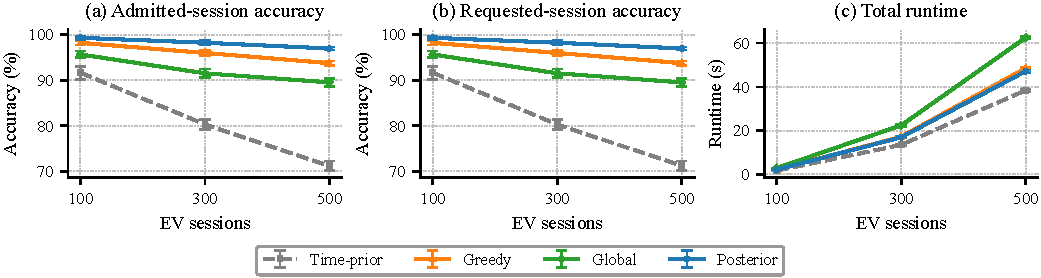
\includegraphics[width=\textwidth,keepaspectratio]{figure3_base_load_comparison.pdf}}
        \caption{The Posterior matcher retains the highest identification accuracy for both admitted and requested sessions as the total session load increases from 100 to 500 sessions, while the time-prior baseline degrades under larger candidate ambiguity; Greedy and Posterior have comparable total runtime, whereas the Global matcher has the highest total runtime (TABLE~\ref{table6}).}
        \label{fig05}
    \end{figure*}

    \section{RESULTS AND DISCUSSION}

    This section reports the comparative evaluation of the four matchers inside the shared event-driven runtime of Sections~III--V.
    The Global baseline transfers the prior MCCT-style correlation--DTW static cost into this online prefix-based decisioning regime, so the comparison isolates the effect of cost-construction and two-stage posterior evidence integration under identical maturity, gating, and finalization timing.

    \subsection{Base-Load Performance}
    The Posterior matcher attains the highest identification accuracy across all evaluated EV-session counts.
    Fig.~\ref{fig05} reports accuracy for $EV \in \{100, 300, 500\}$, where the Posterior matcher reaches $0.99$, $0.98$, and $0.97$ respectively.
    The ranking among the four design families---timing-only, greedy single-shot, correlation-plus-DTW global, and posterior-based assignment---is stable across the EV-session-count sweep.

    At $EV = 500$, the Posterior matcher reduces the misidentification rate from $6.3\,\%$ (greedy) to $3.0\,\%$, and from $10.5\,\%$ (global) to $3.0\,\%$ ($51\,\%$ and $71\,\%$ relative reductions).
    These reductions reflect posterior-based cost construction rather than a tighter single-shot metric.
    Notably, the Global matcher ($0.90$) trails the simpler Greedy matcher ($0.94$), consistent with its multiplicative correlation--DTW score having been designed for complete static waveforms rather than the truncated, noise-perturbed prefixes visible at the watermark instant; transferring the prior MCCT-style static cost directly into the online prefix regime is thus not by itself sufficient.
    The time-prior baseline reaches $0.71$ because the candidate-time gate ($\Delta = 120$\,s) restricts each EV to an operationally plausible candidate set, so timing alone resolves many cases; the remaining $29\,\%$ is where waveform evidence becomes decisive.

    The accuracy advantage is obtained under identical decision timing: every matcher uses the same maturity and evaluation-tick rule, so the 90th-percentile decision latency is $416\,\text{s}$ for all four methods.
    Finalization can occur after the nominal $t_{\text{wm},i}=t_{\text{eff},i}+d_{\max}$ because the relevant EV-side sample must be generated, sensed, ingested, and processed at the next evaluation tick.
    At $EV = 500$, the Greedy and Posterior matchers have similar total runtimes while the Global matcher is slower (TABLE~\ref{table6}), and cost construction dominates over fallback handling, so the accuracy improvement does not result from additional waiting.
    The requested-session accuracy dispersion across the evaluation repeats is small relative to the inter-matcher gaps.

    \begin{table*}[t!]
        \caption{The Posterior matcher achieves the highest accuracy at the representative operating point under identical decision timing (mean over 20 paired repeats; $\pm$ denotes 95\,\% confidence interval; requested-session accuracy coincides with overall accuracy (no blocking) with the same interval).}
        \label{table6}
        \centering
        \begin{tabular}{lcccc}
            \toprule
            \textbf{Matcher} & \textbf{Overall identification accuracy} & \textbf{Requested-session accuracy} & \textbf{90th-percentile decision latency (s)} & \textbf{Total runtime (s)} \\
            \midrule
            Time-prior & 0.71 $\pm$ 0.01 & 0.71 & 416 & 38.4 \\
            Greedy & 0.94 $\pm$ 0.01 & 0.94 & 416 & 48.5 \\
            Global & 0.90 $\pm$ 0.01 & 0.90 & 416 & 62.5 \\
            \textbf{Posterior} & \textbf{0.97 $\pm$ 0.003} & \textbf{0.97} & 416 & 47.1 \\
            \bottomrule
        \end{tabular}
    \end{table*}

    \subsection{Robustness Across Operating Sweeps}

    The ranking of matchers persists across the three evaluated sweep axes, indicating that the measured advantage of the Posterior matcher is not tied to a single default configuration.

    \textbf{EV sampling period.}
    The ranking is preserved at every sampling period within the evaluated range (Fig.~\ref{fig06}).
    Across $\Delta t_{\text{EV}} \in \{5, 15, 30\}$\,s at $EV = 500$, the Posterior matcher attains $0.95$, $0.96$, and $0.97$, respectively. Under the fixed ingestion and sensing assumptions of Section~V-A, this nondecreasing trend suggests that denser sampling adds more noise-perturbed points to the truncated prefix without adding decision-relevant structure.
    Its advantage over the greedy waveform baseline remains within a narrow band of $0.02$--$0.03$.

    \begin{figure}[!t]
        \centerline{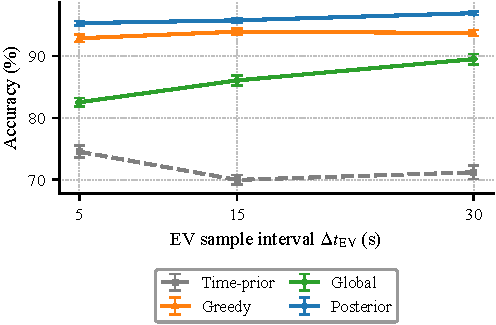
\includegraphics[width=\columnwidth,keepaspectratio]{figure4_sampling_sensitivity.pdf}}
        \caption{The ordering among matchers is preserved across three EV sampling periods at $EV = 500$, indicating that the measured advantage of the Posterior matcher is not specific to a single sampling configuration.}
        \label{fig06}
    \end{figure}

    \textbf{Watermark and candidate margin.}
    Moderate watermark values are sufficient under the present ingestion model.
    At $EV = 500$, the three non-trivial matchers remain stable across $d_{\max} \in \{5, 10, 15\}$\,s, with variation less than $0.01$.
    The time-prior baseline stays near $0.70$ over the same range.
    The Posterior matcher moves only from $0.96$ at $\Delta = 60$\,s to $0.97$ at $120$\,s and stabilizes at $0.97$ through $180$\,s.
    The temporal gate in Eq.~\eqref{eq:e4} retains the ground-truth slot for all admitted sessions in the evaluated envelope ($\approx$28 candidates per EV on average at the representative $\Delta = 120$\,s, with no fallback-to-all activations).
    The $\Delta$ sensitivity above therefore reflects matcher discrimination rather than upstream candidate loss.

    \textbf{Sensing parameters and high-load stress.}
    Sensitivity to the EV-side sensing parameters and to high-load stress is not separately evaluated within the present envelope.
    The reported accuracy is obtained under the sensing-distortion defaults of Section~V-A, so the results are conditional on these assumed EV-side degradation settings. A systematic sensing-parameter sweep is left to future work because a field-faithful sweep requires per-EV and per-battery-management-system (BMS) sensing calibration beyond the present study, whose signal basis is a single Wallbox--Tesla equipment pair. A high-load stress sweep with the fifty EVSE slots held fixed is likewise designated as future work in Section~VII.

    \subsection{Ablation and Discussion}
    Residual error stems from candidate-set ambiguity rather than from runtime-timing pathologies.
    A representative success case, the session traced in Fig.~\ref{fig07}, reaches its full-window effective end at $t_{\text{eff}}=360$\,s after arrival and becomes mature at $t_{\text{wm}}=370$\,s (Eq.~\eqref{eq:e2}).
    Success and failure cases alike are finalized through the ordinary watermark path, and their latency differences reflect the sessions' $t_{\text{eff}}$ rather than any matcher-side early commitment, indicating that ordinary online finalization suffices under base load.

    The diagnostic index is not a runtime decision-tick sequence; it records how the top-1 and top-2 posterior scores separate across the checkpoint updates of a single watermark decision: three checkpoints per stage, taken after the carry-over, time-prior, and current-likelihood factors of Eq.~\eqref{eq:e10}.
    This posterior-based scoring is the basis for the Posterior matcher's advantage over single-shot scorers.

    \begin{figure}[!t]
        \centerline{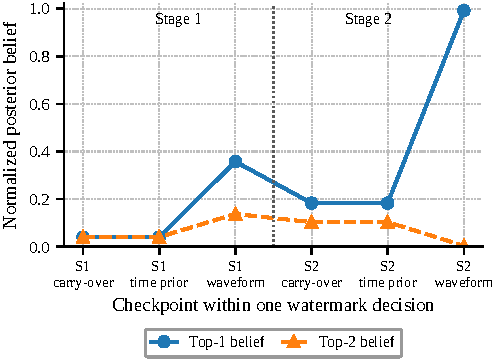
\includegraphics[width=\columnwidth]{figure5_posterior_diagnostic.pdf}}
        \caption{Two-stage posterior evolution of a representative session at the representative operating point ({\unboldmath$EV=500$}). The six diagnostic indices are checkpoint posteriors recorded within the two update stages of a single watermark decision (Section~IV-B), not additional finalization times or runtime decision ticks.}
        \label{fig07}
    \end{figure}

    Ablation identifies the components responsible for the observed behavior (Fig.~\ref{fig08}): for the greedy waveform matcher the full cost is strongest, with the step-signature-removed and DTW-removed variants falling below it and the all-removed variant, which degenerates to the timing-only cost, degrading most as the EV-session count grows; for the global waveform assignment the full score is likewise strongest, with removing correlation causing the larger drop and removing DTW a smaller one; for the Posterior matcher the within-decision posterior carry-over is the decisive component: removing it collapses accuracy to the greedy-baseline level (0.94 at EV{\,}={\,}500), while removing the shaped time prior shifts accuracy by less than the repeat confidence interval.

    \begin{figure*}[!t]
        \centerline{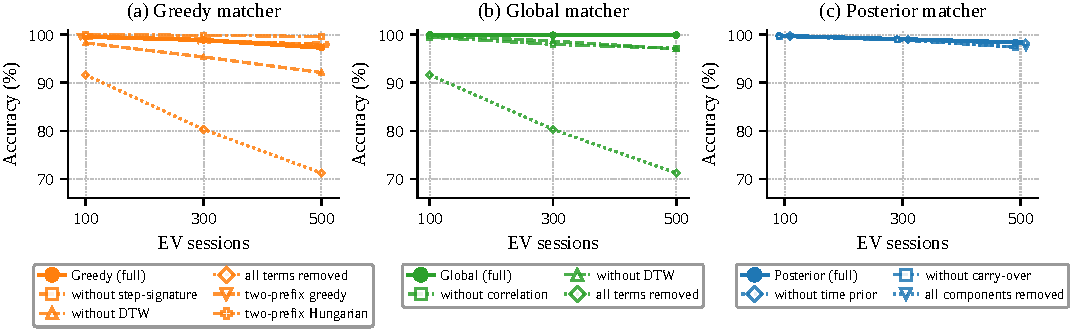
\includegraphics[width=\textwidth]{figure6_ablation_summary.pdf}}
        \caption{Ablation results for the three matcher families, computed on the evaluation repeats of TABLE~\ref{table:calib_eval} (20 paired repeats at {\unboldmath$EV \in \{100, 500\}$}, 15 held-out repeats at {\unboldmath$EV{\,}={\,}300$}). In the Posterior family the within-decision posterior carry-over is the decisive component: removing it, or all posterior components, collapses accuracy to the greedy-baseline level, while the time-prior curve stays within the repeat confidence interval of the full design. Markers of overlapping curves are offset horizontally for visibility.}
        \label{fig08}
    \end{figure*}

    The residual misidentification stems from sequential discrimination among plausible candidates under delayed anonymous telemetry, not from candidate recovery or decision timing: the gate in Eq.~\eqref{eq:e4} retains the ground-truth slot throughout the studied regime, decision latency is shared across methods, and widening the margin or lengthening the watermark changes accuracy only modestly. The Posterior matcher is structurally aligned with the online problem because timing and waveform evidence are integrated within the same watermark-visible decision window, while the greedy waveform baseline remains the strongest simpler alternative when posterior-update state management is undesirable.

    \looseness=1 The reported envelope rests on three layers with decreasing empirical grounding: the charging-current generation model from Nomura~\textit{et al.}~\cite{b14}; the cloud-ingestion model anchored by TABLE~\ref{table3} (transport standards, broadband measurements, OCPP defaults); and an EV-side sensing-distortion layer set to conservative defaults and not calibrated against a specific EV model. The study is therefore framed as a methodology investigation, bounded to a single fifty-slot site with an EVSE response model fitted to one Wallbox--Tesla combination. Adversarial spoofing and timing attacks and adapted classical sequential-association baselines are excluded, the latter because they presuppose time-synchronous, spatially resolved observations (Section~II-C). These, together with multi-site operation and security-hardened deployment, are designated as future work in Section~VII.

    \section{CONCLUSION}
    \looseness=1 This paper extended the measurement-based Wallbox--Tesla current-generation model of prior MCCT work~\cite{b14} into an event-driven online runtime, in which EV sessions arrive and depart asynchronously and EV-side observations reach the backend as delayed anonymous telemetry.
    Unlike static batch assignment over completed waveforms, the resulting decision problem requires irrevocable finalization from a maturing prefix of EV-side evidence under a watermark-governed maturity rule and time-tolerance candidate gating.
    The proposed two-stage Bayesian posterior matcher combines timing and waveform evidence through sequential posterior updates within each watermark decision; in a representative 500-session scenario it attains an identification accuracy of 0.97, outperforming the timing-only, greedy waveform, and prior MCCT-style global waveform baselines under identical decision timing, with the advantage preserved across the evaluated sampling-period, watermark-delay, and candidate-margin settings.
    Ablation attributes the advantage to sequential posterior integration across the two within-decision update stages rather than to any single similarity metric, indicating that extending current-modulation identification to cloud-connected legacy AC operation requires not only waveform similarity but also online integration of delayed evidence.
    Future work should address field-calibrated ingestion-delay and packet-loss models, heterogeneous charger and EV responses, waveform-spoofing threat models, sensitivity to EV-side sensing parameters and high-load saturation, and explicit latency--accuracy stopping rules for early finalization.

    \section*{CODE AVAILABILITY}
    The source code used in this study is publicly available at \url{https://github.com/SmartGridLab/Posterior-Aware-Online-Matching-of-EV-Charger-Pairs-under-Delayed-Anonymous-Telemetry}; the repository contains the event-driven simulator, the four matcher implementations, the per-repeat random seeds, and the \texttt{reproduce\_all} driver script that regenerates every number reported in Section~VI.

    \section*{ACKNOWLEDGMENT}
    The formulation reuses the charging-current generation model of Nomura~\textit{et al.}~\cite{b14}; the EV-side response-lag settings are treated as waveform-generation delays informed by the FAT measurements reported by Imanaka and Baba~\cite{bimanaka25}, while backend telemetry ingestion is modeled separately. The original MCCT proposal by Baba and Imanaka~\cite{b13} is acknowledged as the conceptual origin of this line of work.

    \begingroup
    \scriptsize
    \sloppy
    \emergencystretch=2em
    \tolerance=3000
    \hbadness=10000
    \begin{thebibliography}{40}
    \setlength{\itemsep}{0pt}\setlength{\parsep}{0pt}\setlength{\parskip}{0pt}
                \bibitem{biea26} International Energy Agency, \textit{Global EV Outlook 2026}, Paris, France, 2026. [Online]. Available: \url{https://www.iea.org/reports/global-ev-outlook-2026}

        \bibitem{b2} F. Ahmed, S. Ahmad, M. T. Rahman, M. R. Hazari, R. Faiz, T. Ahmed, and M. Karimi, ``A holistic review of electric vehicle charging impacts on power distribution networks: Technical challenges, smart mitigation strategies and future directions,'' \textit{Appl. Energy}, vol.~402, art.~no.~126961, 2026, doi:~10.1016/j.apenergy.2025.126961.

        \bibitem{b3} S. Powell, G. V. Cezar, L. Min, I. M. L. Azevedo, and R. Rajagopal, ``Charging infrastructure access and operation to reduce the grid impacts of deep electric vehicle adoption,'' \textit{Nat. Energy}, vol.~7, no.~10, pp.~932--945, Oct.~2022.

        \bibitem{b5} P. V. Dahiwale, Z. H. Rather, and I. Mitra, ``A comprehensive review of smart charging strategies for electric vehicles and way forward,'' \textit{IEEE Trans. Intell. Transp. Syst.}, vol.~25, no.~9, pp.~10462--10482, Sep.~2024, doi:~10.1109/TITS.2024.3365581.

        \bibitem{b8} S. S. G. Acharige, M. E. Haque, M. T. Arif, N. Hosseinzadeh, K. N. Hasan, and A. M. T. Oo, ``Review of electric vehicle charging technologies, standards, architectures, and converter configurations,'' \textit{IEEE Access}, vol.~11, pp.~41218--41255, 2023.

        \bibitem{biec} International Electrotechnical Commission, \textit{IEC 61851-1:2019, Electric Vehicle Conductive Charging System --- Part 1: General Requirements}, Geneva, Switzerland, 2019.

        \bibitem{b6} H. S. Das, M. M. Rahman, S. Li, and C. W. Tan, ``Electric vehicles standards, charging infrastructure, and impact on grid integration: A technological review,'' \textit{Renew. Sustain. Energy Rev.}, vol.~120, art.~no.~109618, Mar.~2020.

        \bibitem{b7} International Organization for Standardization, \textit{ISO 15118-20:2022, Road Vehicles --- Vehicle to Grid Communication Interface --- Part 20: 2nd Generation Network and Application Protocol Requirements}, Geneva, Switzerland, 2022.

        \bibitem{b13} H. Baba and M. Imanaka, ``Report on basic experiments of normal charger-EV linking technology,'' in \textit{Proc. IEEJ EIS Division Conf.}, Paper GS8-6, Aug. 2024.

        \bibitem{b14} N. Nomura, M. Imanaka, H. Baba, and D. Kodaira, ``Individual identification of multiple EV--charger pairs via modulated charging current technology,'' in \textit{Proc. 14th Int. Conf. Renewable Energy Research and Applications (ICRERA)}, Vienna, Austria, Oct.~2025, pp.~246--251, doi:~10.1109/ICRERA66237.2025.11283721.

        \bibitem{b15} H. W. Kuhn, ``The Hungarian method for the assignment problem,'' \textit{Naval Res. Logist. Quart.}, vol.~2, no.~1--2, pp.~83--97, 1955.

        \bibitem{b26} T. Akidau \textit{et al.}, ``The Dataflow model: A practical approach to balancing correctness, latency, and cost in massive-scale, unbounded, out-of-order data processing,'' \textit{Proc. VLDB Endow.}, vol.~8, no.~12, pp.~1792--1803, 2015.

        \bibitem{bhart} G. W. Hart, ``Nonintrusive appliance load monitoring,'' \textit{Proc. IEEE}, vol.~80, no.~12, pp.~1870--1891, Dec.~1992.

        \bibitem{b9} A. M. A. Haidar and K. M. Muttaqi, ``Behavioral characterization of electric vehicle charging loads in a distribution power grid through modeling of battery chargers,'' \textit{IEEE Trans. Ind. Appl.}, vol.~52, no.~1, pp.~483--492, Jan.--Feb.~2016, doi:~10.1109/TIA.2015.2483705.

        \bibitem{b10} F. Ferretti and A. De~Paola, ``Machine learning identification of electric vehicles from charging session data,'' \textit{Energy AI}, vol.~20, art.~no.~100502, May~2025, doi:~10.1016/j.egyai.2025.100502.

        \bibitem{b11} A. Brighente, M. Conti, D. Donadel, and F. Turrin, ``EVScout2.0: Electric vehicle profiling through charging profile,'' \textit{ACM Trans. Cyber-Phys. Syst.}, vol.~8, no.~2, art.~no.~11, Apr.~2024, doi:~10.1145/3565268.

        \bibitem{b12} S. Matrone, E. G. C. Ogliari, A. Nespoli, G. Gruosso, and A. Gandelli, ``Electric vehicles charging sessions classification technique for optimized battery charge based on machine learning,'' \textit{IEEE Access}, vol.~11, pp.~52444--52451, 2023.

        \bibitem{bmarchiori25} F. Marchiori, D. Donadel, A. Brighente, and M. Conti, ``Profiling electric vehicles via early charging voltage patterns,'' presented at the \textit{AI \& CPSS Workshop, Int. Conf. Availability, Reliability and Security (ARES)}, Ghent, Belgium, Aug.~2025. [Online]. Available: \url{https://arxiv.org/abs/2506.07714}

        \bibitem{bferretti24} F. Ferretti, A. De~Paola, H. Scholz, S. Tarantola, and E. Kotsakis, ``Reference power tracking for AC charging of electric vehicles,'' \textit{IEEE Access}, vol.~12, pp.~174245--174254, 2024, doi:~10.1109/ACCESS.2024.3501474.

        \bibitem{b20} W. Kim, P.-Y. Lee, J. Kim, and K.-S. Kim, ``A robust state of charge estimation approach based on nonlinear battery cell model for lithium-ion batteries in electric vehicles,'' \textit{IEEE Trans. Veh. Technol.}, vol.~70, no.~6, pp.~5638--5647, Jun.~2021, doi:~10.1109/TVT.2021.3079934.

        \bibitem{b21} M. Pasetti, S. Dello~Iacono, and D. Zaninelli, ``Real-time state of charge estimation of light electric vehicles based on active power consumption,'' \textit{IEEE Access}, vol.~11, pp.~110995--111010, 2023, doi:~10.1109/ACCESS.2023.3322651.

        \bibitem{bkhanda} A. Khanda, A. Satpathy, and S. K. Das, ``SMART-CHARGE: Stable matching algorithm for electric vehicle charging in subscription-based models,'' \textit{Pervasive Mobile Comput.}, vol.~118, art.~no.~102197, May~2026, doi:~10.1016/j.pmcj.2026.102197.

        \bibitem{breactttc} A. Satpathy, A. Khanda, C. Swain, and S. K. Das, ``ReACT-TTC: Capacity-aware top trading cycles for post-choice reassignment in shared CPS,'' presented at the \textit{17th ACM/IEEE Int. Conf. Cyber-Physical Syst. (ICCPS)}, Saint-Malo, France, May~2026. [Online]. Available: \url{https://arxiv.org/abs/2602.00859}, doi:~10.48550/arXiv.2602.00859.

        \bibitem{b17} R. M. Karp, U. V. Vazirani, and V. V. Vazirani, ``An optimal algorithm for on-line bipartite matching,'' in \textit{Proc. 22nd ACM Symp. Theory of Computing (STOC)}, 1990, pp.~352--358.

        \bibitem{b18} A. Mehta, ``Online matching and ad allocation,'' \textit{Found. Trends Theor. Comput. Sci.}, vol.~8, no.~4, pp.~265--368, 2013.

        \bibitem{bemek16} Y. Emek, S. Kutten, and R. Wattenhofer, ``Online matching: Haste makes waste!,'' in \textit{Proc. 48th Annu. ACM Symp. Theory Comput. (STOC)}, Cambridge, MA, USA, Jun.~2016, pp.~333--344, doi:~10.1145/2897518.2897557.

        \bibitem{b19} Y. Bar-Shalom, X. R. Li, and T. Kirubarajan, \textit{Estimation with Applications to Tracking and Navigation}. New York, NY, USA: Wiley, 2001.

        \bibitem{bsarkka} S. S\"{a}rkk\"{a}, \textit{Bayesian Filtering and Smoothing}. Cambridge, U.K.: Cambridge Univ. Press, 2013.

        \bibitem{b22} Open Charge Alliance, \textit{Open Charge Point Protocol 2.0.1, Part~2 --- Specification}, Arnhem, The Netherlands, 2020. [Online]. Available: \url{https://openchargealliance.org/protocols/ocpp-201/}

        \bibitem{b23} I. Fette and A. Melnikov, ``The WebSocket Protocol,'' Internet Engineering Task Force, RFC~6455, Dec.~2011.

        \bibitem{b24} V. Paxson, M. Allman, J. Chu, and M. Sargent, ``Computing TCP's Retransmission Timer,'' Internet Engineering Task Force, RFC~6298, Jun.~2011.

        \bibitem{b25} Federal Communications Commission, \textit{Measuring Fixed Broadband---Thirteenth Report}, Washington, DC, USA, Aug.~2024. [Online]. Available: \url{https://www.fcc.gov/reports-research/reports/measuring-broadband-america/measuring-fixed-broadband-thirteenth-report}

        \bibitem{bimanaka23} M. Imanaka, Y. Ishida, H. Baba, and W. Hirohashi, ``Prototyping reference model for combined behavior of ICT systems and energy equipment'' (in Japanese), \textit{Seisan-Kenkyu (J. Inst. Industrial Sci., Univ. of Tokyo)}, vol.~75, no.~4, pp.~333--341, 2023.

        \bibitem{bsatya} M. Satyanarayanan, ``The emergence of edge computing,'' \textit{Computer}, vol.~50, no.~1, pp.~30--39, Jan.~2017.

        \bibitem{b16} H. Sakoe and S. Chiba, ``Dynamic programming algorithm optimization for spoken word recognition,'' \textit{IEEE Trans. Acoust., Speech, Signal Process.}, vol.~26, no.~1, pp.~43--49, 1978.

        \bibitem{bimanaka25} M. Imanaka and H. Baba, ``Measurement of both full activation time and ICT response time for fast demand response of electric vehicle charging,'' \textit{IEEJ Trans. Electr. Electron. Eng.}, vol.~21, no.~2, pp.~307--315, Feb.~2026, doi:~10.1002/tee.70176.

        \bibitem{bzaptec} Zaptec, \textit{Zaptec Go2 OCPP 1.6J Supported Configuration Keys}. [Online]. Available: \url{https://docs.zaptec.com/docs/zaptec-go2-ocpp-16j-supported-configuration-keys}

        \bibitem{babb} ABB, \textit{Terra AC Wallbox --- OCPP Configuration Guide}, document 9AKK107992A1326. [Online]. Available: \url{https://forum.iobroker.net/assets/uploads/files/1658735175644-9akk107992a1326_terraac-chargepointconfigurationocpp.pdf}

\end{thebibliography}
    \endgroup

    \begin{IEEEbiography}[{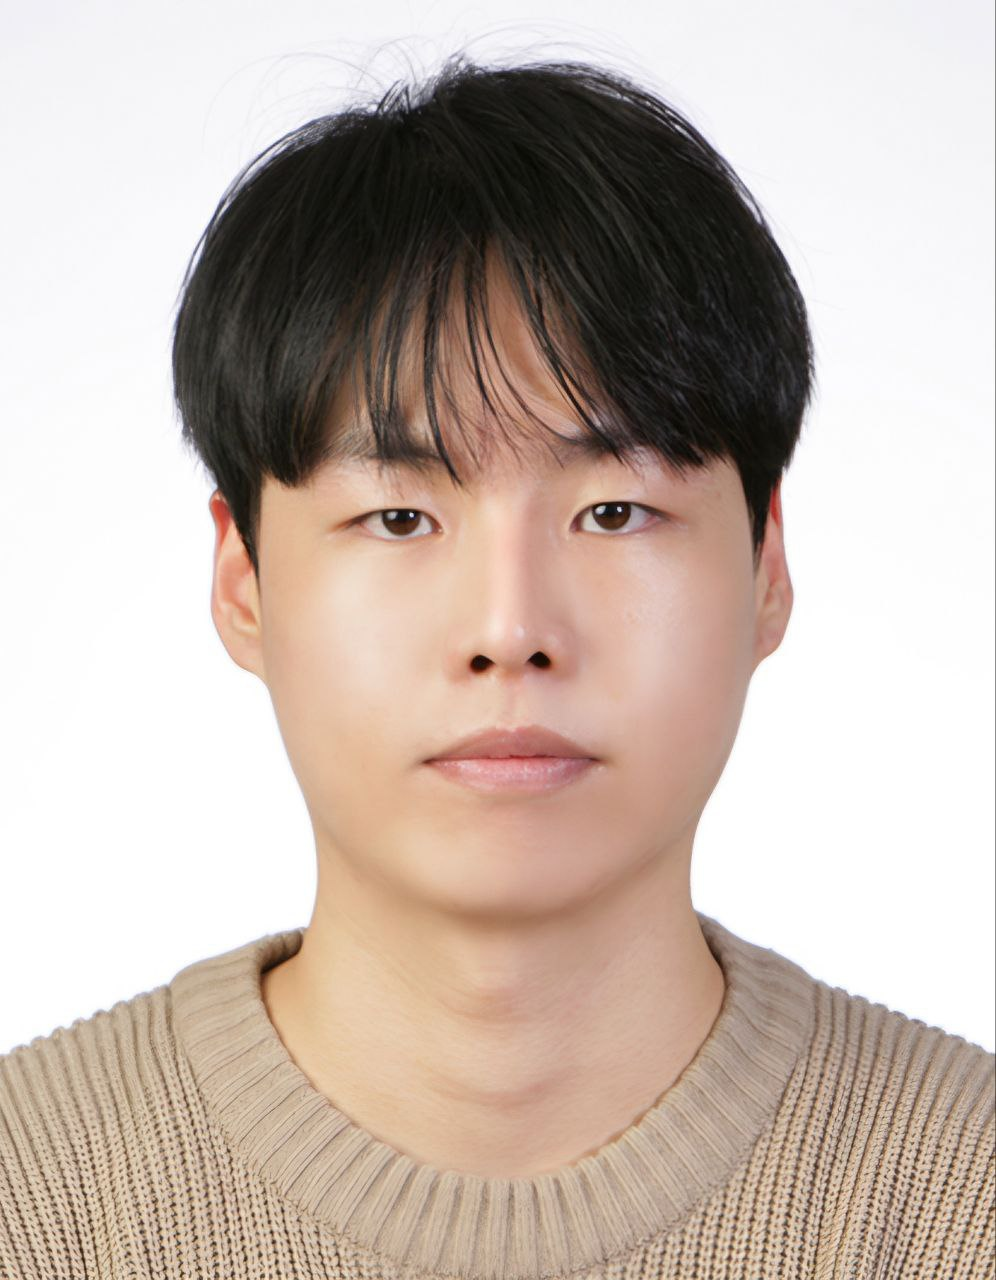
\includegraphics[width=1in,height=1.25in,clip,keepaspectratio]{author1_yang.png}}]{Jiseok Yang} received the B.S.\ degree in electrical and electronic engineering from Chungbuk National University, Cheongju, South Korea, in 2025. He is currently pursuing the M.S.\ degree in systems and information engineering with the University of Tsukuba, Japan. His research interests include EV charging, asynchronous cloud telemetry, and online matching and identification for cyber-physical systems, with a current focus on Bayesian posterior tracking under partial and delayed observability.
    \end{IEEEbiography}
    \begin{IEEEbiography}[{
\includegraphics[width=1in,height=1.25in,clip,keepaspectratio]{author2_kodaira.png}}]{Daisuke Kodaira} (Member,~IEEE) received the Ph.D.\ degree in electrical engineering from Tokyo Metropolitan University, Japan. He is an Associate Professor with the Institute of Systems and Information Engineering, University of Tsukuba, Japan, with research interests in intelligent transportation systems, mobility-data platforms, EV charging infrastructure, and cyber-physical integration.
    \end{IEEEbiography}

    \EOD

\end{document}
